%<dscrpt>Fichier de déclarations Latex à inclure au début d'un élément de cours.</dscrpt>

\documentclass[a4paper]{article}
\usepackage[hmargin={1.8cm,1.8cm},vmargin={2.4cm,2.4cm},headheight=13.1pt]{geometry}

%includeheadfoot,scale=1.1,centering,hoffset=-0.5cm,
\usepackage[pdftex]{graphicx,color}
\usepackage[french]{babel}
%\selectlanguage{french}
\addto\captionsfrench{
  \def\contentsname{Plan}
}
\usepackage{fancyhdr}
\usepackage{floatflt}
\usepackage{amsmath}
\usepackage{amssymb}
\usepackage{amsthm}
\usepackage{stmaryrd}
%\usepackage{ucs}
\usepackage[utf8]{inputenc}
%\usepackage[latin1]{inputenc}
\usepackage[T1]{fontenc}


\usepackage{titletoc}
%\contentsmargin{2.55em}
\dottedcontents{section}[2.5em]{}{1.8em}{1pc}
\dottedcontents{subsection}[3.5em]{}{1.2em}{1pc}
\dottedcontents{subsubsection}[5em]{}{1em}{1pc}

\usepackage[pdftex,colorlinks={true},urlcolor={blue},pdfauthor={remy Nicolai},bookmarks={true}]{hyperref}
\usepackage{makeidx}

\usepackage{multicol}
\usepackage{multirow}
\usepackage{wrapfig}
\usepackage{array}
\usepackage{subfig}


%\usepackage{tikz}
%\usetikzlibrary{calc, shapes, backgrounds}
%pour la présentation du pseudo-code
% !!!!!!!!!!!!!!      le package n'est pas présent sur le serveur sous fedora 16 !!!!!!!!!!!!!!!!!!!!!!!!
%\usepackage[french,ruled,vlined]{algorithm2e}

%pr{\'e}sentation du compteur de niveau 2 dans les listes
\makeatletter
\renewcommand{\labelenumii}{\theenumii.}
\renewcommand{\thesection}{\Roman{section}.}
\renewcommand{\thesubsection}{\arabic{subsection}.}
\renewcommand{\thesubsubsection}{\arabic{subsubsection}.}
\makeatother


%dimension des pages, en-t{\^e}te et bas de page
%\pdfpagewidth=20cm
%\pdfpageheight=14cm
%   \setlength{\oddsidemargin}{-2cm}
%   \setlength{\voffset}{-1.5cm}
%   \setlength{\textheight}{12cm}
%   \setlength{\textwidth}{25.2cm}
   \columnsep=1cm
   \columnseprule=0.5pt

%En tete et pied de page
\pagestyle{fancy}
\lhead{MPSI-\'Eléments de cours}
\rhead{\today}
%\rhead{25/11/05}
\lfoot{\tiny{Cette création est mise à disposition selon le Contrat\\ Paternité-Pas d'utilisations commerciale-Partage des Conditions Initiales à l'Identique 2.0 France\\ disponible en ligne http://creativecommons.org/licenses/by-nc-sa/2.0/fr/
} }
\rfoot{\tiny{Rémy Nicolai \jobname}}


\newcommand{\baseurl}{http://back.maquisdoc.net/data/cours\_nicolair/}
\newcommand{\urlexo}{http://back.maquisdoc.net/data/exos_nicolair/}
\newcommand{\urlcours}{https://maquisdoc-math.fra1.digitaloceanspaces.com/}

\newcommand{\N}{\mathbb{N}}
\newcommand{\Z}{\mathbb{Z}}
\newcommand{\C}{\mathbb{C}}
\newcommand{\R}{\mathbb{R}}
\newcommand{\D}{\mathbb{D}}
\newcommand{\K}{\mathbf{K}}
\newcommand{\Q}{\mathbb{Q}}
\newcommand{\F}{\mathbf{F}}
\newcommand{\U}{\mathbb{U}}
\newcommand{\p}{\mathbb{P}}


\newcommand{\card}{\mathop{\mathrm{Card}}}
\newcommand{\Id}{\mathop{\mathrm{Id}}}
\newcommand{\Ker}{\mathop{\mathrm{Ker}}}
\newcommand{\Vect}{\mathop{\mathrm{Vect}}}
\newcommand{\cotg}{\mathop{\mathrm{cotan}}}
\newcommand{\sh}{\mathop{\mathrm{sh}}}
\newcommand{\ch}{\mathop{\mathrm{ch}}}
\newcommand{\argsh}{\mathop{\mathrm{argsh}}}
\newcommand{\argch}{\mathop{\mathrm{argch}}}
\newcommand{\tr}{\mathop{\mathrm{tr}}}
\newcommand{\rg}{\mathop{\mathrm{rg}}}
\newcommand{\rang}{\mathop{\mathrm{rg}}}
\newcommand{\Mat}{\mathop{\mathrm{Mat}}}
\newcommand{\MatB}[2]{\mathop{\mathrm{Mat}}_{\mathcal{#1}}\left( #2\right) }
\newcommand{\MatBB}[3]{\mathop{\mathrm{Mat}}_{\mathcal{#1} \mathcal{#2}}\left( #3\right) }
\renewcommand{\Re}{\mathop{\mathrm{Re}}}
\renewcommand{\Im}{\mathop{\mathrm{Im}}}
\renewcommand{\th}{\mathop{\mathrm{th}}}
\newcommand{\repere}{$(O,\overrightarrow{i},\overrightarrow{j},\overrightarrow{k})$}
\newcommand{\cov}{\mathop{\mathrm{Cov}}}

\newcommand{\absolue}[1]{\left| #1 \right|}
\newcommand{\fonc}[5]{#1 : \begin{cases}#2 \rightarrow #3 \\ #4 \mapsto #5 \end{cases}}
\newcommand{\depar}[2]{\dfrac{\partial #1}{\partial #2}}
\newcommand{\norme}[1]{\left\| #1 \right\|}
\newcommand{\se}{\geq}
\newcommand{\ie}{\leq}
\newcommand{\trans}{\mathstrut^t\!}
\newcommand{\val}{\mathop{\mathrm{val}}}
\newcommand{\grad}{\mathop{\overrightarrow{\mathrm{grad}}}}

\newtheorem*{thm}{Théorème}
\newtheorem{thmn}{Théorème}
\newtheorem*{prop}{Proposition}
\newtheorem{propn}{Proposition}
\newtheorem*{pa}{Présentation axiomatique}
\newtheorem*{propdef}{Proposition - Définition}
\newtheorem*{lem}{Lemme}
\newtheorem{lemn}{Lemme}

\theoremstyle{definition}
\newtheorem*{defi}{Définition}
\newtheorem*{nota}{Notation}
\newtheorem*{exple}{Exemple}
\newtheorem*{exples}{Exemples}


\newenvironment{demo}{\renewcommand{\proofname}{Preuve}\begin{proof}}{\end{proof}}
%\renewcommand{\proofname}{Preuve} doit etre après le begin{document} pour fonctionner

\theoremstyle{remark}
\newtheorem*{rem}{Remarque}
\newtheorem*{rems}{Remarques}

\renewcommand{\indexspace}{}
\renewenvironment{theindex}
  {\section*{Index} %\addcontentsline{toc}{section}{\protect\numberline{0.}{Index}}
   \begin{multicols}{2}
    \begin{itemize}}
  {\end{itemize} \end{multicols}}


%pour annuler les commandes beamer
\renewenvironment{frame}{}{}
\newcommand{\frametitle}[1]{}
\newcommand{\framesubtitle}[1]{}

\newcommand{\debutcours}[2]{
  \chead{#1}
  \begin{center}
     \begin{huge}\textbf{#1}\end{huge}
     \begin{Large}\begin{center}Rédaction incomplète. Version #2\end{center}\end{Large}
  \end{center}
  %\section*{Plan et Index}
  %\begin{frame}  commande beamer
  \tableofcontents
  %\end{frame}   commande beamer
  \printindex
}


\makeindex
\begin{document}
\noindent

\debutcours{Suites définies par récurrence}{alpha}

Obsolète transféré dans le cours sur les fonctions dérivables
Cette section ne fait pas partie du programme de la classe de MPSI. Les résultats présentés ne doivent donc pas être utilisés directement surtout à l'écrit. L'objectif est de dégager certaines situations caractéristiques.

Le contexte général est l'étude de suites vérifiant une relation de récurrence du ype
\begin{displaymath}
 x_{n+1}=f(x_n)
\end{displaymath}
où $f$ est une fonction définie dans une partie de $\R$ et à valeurs réelles.

Les résultats présentés ici ne couvrent que des cas très particuliers et ne représentent absolument pas la complexité de la question.
\section{Vocabulaire - Résultats généraux}
\begin{defi}
 On dira qu'un intervalle $I$ est stable \index{intervalle stable} pour une fonction $f$ lorsque $I$ est inclus dans l'espace de départ de $f$ et que $f(I)\subset I$.\newline
On dira que $a$ appartenant à l'espace de départ d'une fonction $f$ est un \emph{point fixe} de $f$ lorsque $f(a)=a$.  
\end{defi}
\begin{prop}
 Lorsque $I$ est un intervalle stable pour $f$, pour toute condition initiale $x_0\in I$, la suite $(x_n)_{n\in \N}$ est définie pour tous les entiers $n$.
\end{prop}
\begin{defi}
 On dira qu'un point fixe $a$ de $f$ est stable (ou attractif) si et seulement si il est à l'intérieur d'un intervalle $J$ stable pour $f$ et tel que, pour toute condition initiale $x_0\in J$, la suite $(x_n)_{n\in \N}$ converge vers $a$.
\end{defi}
\begin{defi}
 On dira qu'un point fixe $a$ de $f$ est stable (ou attractif) si et seulement si il existe un intervalle $J$ stable pour $f$ tel que $a$ est à l'intérieur de $J$ et que, pour toute condition initiale $x_0\in J$, la suite $(x_n)_{n\in \N}$ converge vers $a$.
\end{defi}
\begin{defi}
 On dira qu'un point fixe $a$ de $f$ est instable (ou répulsif) si et seulement si il existe un intervalle $J$ tel que $a$ est à l'intérieur de $J$ et que, pour toute condition initiale $x_0\in J$, il existe un entier $N(x_0)$ tel que :
\begin{displaymath}
 x_0\in J, x_1\in J, \cdots , x_{N(x_0)-1}\in J, x_{N(x_0)} \not \in J
\end{displaymath}
\end{defi}
\begin{prop}
 Lorsque la suite converge vers un réel $a$ dans l'espace de départ de $f$ et que $f$ est continue en $a$, ce point $a$ est un point fixe de $f$.
\end{prop}
\begin{demo}
 En effet, par continuité de $f$ en $a$, $(f(x_{n}))_{n\in \N}$ converge vers $f(a)$ mais cette suite est aussi égale à la suite extraite $(x_{n+1})_{n\in \N}$ qui converge vers $a$.
\end{demo}
\begin{defi}
Le \emph{bassin d'attraction} d'un point fixe $a$ est formé par l'ensemble des conditions initiales $x_0$ pour lesquelles la suite $(x_{n})_{n\in \N}$ converge vers $a$.
\end{defi}

\section{Fonctions monotones}
\subsection{Fonction croissante}
\begin{figure}[h!t]
 \centering
 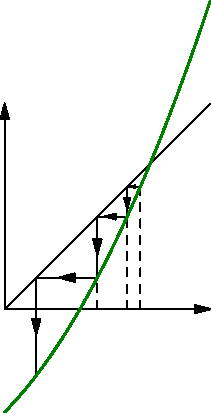
\includegraphics{C4792_1.pdf}
 % C4792_1.pdf: 99x198 pixel, 72dpi, 3.49x6.99 cm, bb=0 0 99 198
 \caption{Divergence monotone}
 \label{fig:C4792_1}
\end{figure}

\begin{prop}
 Lorsque $I$ est un intervalle stable pour $f$ et que $f$ est croissante sur $I$, alors, pour toute condition initiale $x_0\in I$, la suite $(x_n)_{n\in \N}$ est monotone.
\end{prop}
\begin{demo}
 En fait la première inégalité, celle entre les valeurs $x_0$ et $x_1$, va \emph{se propager} par récurrence:
\begin{align*}
 x_0\leq x_1 &\Rightarrow \forall n \in \N : x_n \leq x_{n+1} &:\text{ suite croissante}\\
x_0\geq x_1 &\Rightarrow \forall n \in \N : x_n \geq x_{n+1} &:\text{ suite décroissante}
\end{align*}
\end{demo}
\subsection{Fonction décroissante}
\subsection{Conditions suffisantes de stabilité ou d'instabilité}
Lorsque le signe de $f(x)-x$ est connu dans un intervalle autour d'un point fixe, on peut parfois savoir si ce point est stable ou instable.
\begin{itemize}
 \item Le point fixe est \emph{instable} lorsque la distribution des signes dans un intervalle $J$ est comme dans le tableau suivant :
\begin{center}
 \begin{tabular}{c|ccc|}
   &  & a &  \\  \hline
 f(x)-x   & - & 0 & + \\ \hline
\end{tabular}
\end{center}
Lorsque la fonction est $\mathcal C^1$ dans $J$, la condition $f'(a)>1$ entraine une telle distribution locale des signes.

 \item Le point fixe est \emph{stable} lorsque la distribution des signes dans un intervalle $J$ est comme dans le tableau suivant :
\begin{center}
 \begin{tabular}{c|ccc|}
   &  & a &  \\  \hline
 f(x)-x   & + & 0 & - \\ \hline
\end{tabular}
\end{center}
Lorsque la fonction est $\mathcal C^1$ dans $J$, la condition $0\leq f'(a) < 1$ entraine une telle distribution locale des signes.
\end{itemize}
\begin{rems}
 \begin{itemize}
  \item Méthode de Newton
  \item Application contractante. Toute applcation contractante dans un intervalle stable admet un unique point fixe.
 \end{itemize}

\end{rems}

\section{Expressions particulières}
\subsection{Récurrence arithmético-géométrique}
\subsection{Récurrence homographique}
\subsection{Récurrence linéaire}
\end{document}
